% This file was created by matplotlib2tikz v0.7.4.
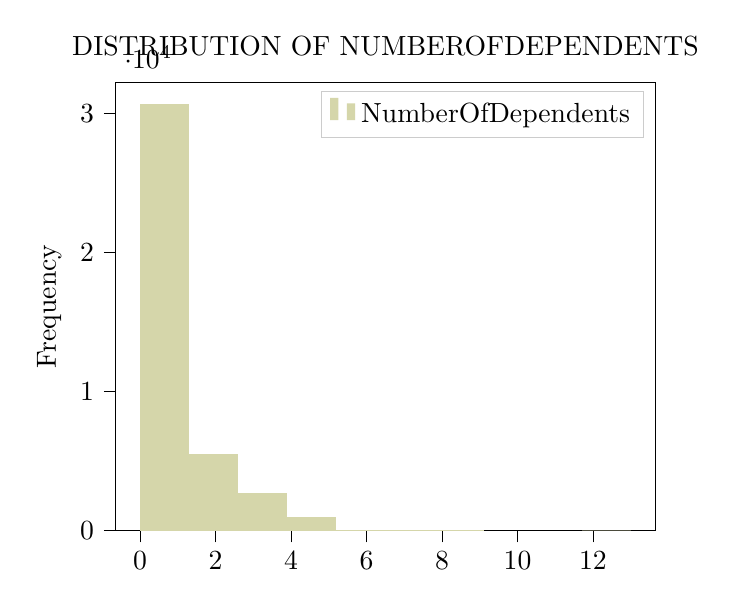
\begin{tikzpicture}

\definecolor{color0}{rgb}{0.835294117647059,0.83921568627451,0.666666666666667}

\begin{axis}[
legend cell align={left},
legend style={draw=white!80.0!black},
tick align=outside,
tick pos=left,
title={\printsubsection{\MakeUppercase{Distribution of NumberOfDependents}}},
x grid style={white!69.01960784313725!black},
xmin=-0.65, xmax=13.65,
xtick style={color=black},
y grid style={white!69.01960784313725!black},
ylabel={Frequency},
ymin=0, ymax=32249.7,
ytick style={color=black}
]
\draw[fill=color0,draw opacity=0] (axis cs:0,0) rectangle (axis cs:1.3,30714);
\addlegendimage{ybar,ybar legend,fill=color0,draw opacity=0};
\addlegendentry{NumberOfDependents}

\draw[fill=color0,draw opacity=0] (axis cs:1.3,0) rectangle (axis cs:2.6,5539);
\draw[fill=color0,draw opacity=0] (axis cs:2.6,0) rectangle (axis cs:3.9,2666);
\draw[fill=color0,draw opacity=0] (axis cs:3.9,0) rectangle (axis cs:5.2,987);
\draw[fill=color0,draw opacity=0] (axis cs:5.2,0) rectangle (axis cs:6.5,51);
\draw[fill=color0,draw opacity=0] (axis cs:6.5,0) rectangle (axis cs:7.8,12);
\draw[fill=color0,draw opacity=0] (axis cs:7.8,0) rectangle (axis cs:9.1,9);
\draw[fill=color0,draw opacity=0] (axis cs:9.1,0) rectangle (axis cs:10.4,0);
\draw[fill=color0,draw opacity=0] (axis cs:10.4,0) rectangle (axis cs:11.7,0);
\draw[fill=color0,draw opacity=0] (axis cs:11.7,0) rectangle (axis cs:13,1);
\end{axis}

\end{tikzpicture}